\section{Three 4-transpositions}

\paragraph{}
Now we use Lemma~\ref{rank-4-3-patterns} to prove the Theorems~\ref{rank4-3-th1} and~\ref{rank4-3-th2}.

\begin{theorem}
  \label{rank4-3-th1}
  All sggis of rank 4 on $A_{11}$ with three 4-transpositions are those displayed in appendix~\ref{rank4-3-4transpositions}.
\end{theorem}

\begin{proof}
  Let, without loss of generality, $\rho_1$ and $\rho_3$ be 4-transpositions.

  \begin{figure}[H]
    \begin{center}
      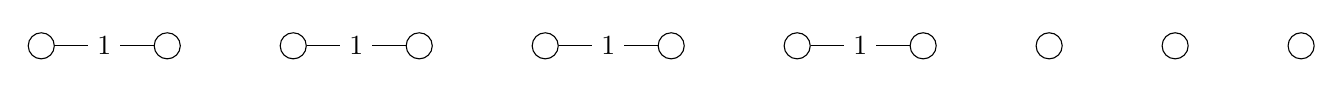
\begin{tikzpicture}[scale=.8]

        \begin{scope}[every node/.style={circle,draw}]
          \node (1)  at (0,0)  {};
          \node (2)  at (2,0)  {};
          \node (3)  at (4,0)  {};
          \node (4)  at (6,0)  {};
          \node (5)  at (8,0)  {};
          \node (6)  at (10,0)  {};
          \node (7)  at (12,0)  {};
          \node (8)  at (14,0)  {};
          \node (9)  at (16,0)  {};
          \node (10) at (18,0)  {};
          \node (11) at (20,0) {};
        \end{scope}

        \begin{scope}[every node/.style={fill=white}]

          \begin{scope}[every edge/.style={draw}]
            \path (1)  edge node {$1$} (2);
            \path (3)  edge node {$1$} (4);
            \path (5)  edge node {$1$} (6);
            \path (7)  edge node {$1$} (8);
          \end{scope}
        \end{scope}

      \end{tikzpicture}
      \caption{}
    \end{center}
  \end{figure}

  \paragraph{}By Lemma~\ref{rank-4-3-patterns}, the pattern between $\rho_1$ and $\rho_3$ is the following.


  \begin{figure}[H]
    \begin{center}
      \begin{tikzpicture}[scale=.8]

        \begin{scope}[every node/.style={circle,draw}]
          \node (1)  at (0,2)  {};
          \node (2)  at (0,0)  {};
          \node (3)  at (2,2)  {};
          \node (4)  at (2,0)  {};
          \node (5)  at (4,0)  {};
          \node (6)  at (6,0)  {};
          \node (7)  at (8,0)  {};
          \node (8)  at (10,0) {};
          \node (9)  at (12,0) {};
          \node (10) at (14,0) {};
          \node (11) at (16,0) {};
        \end{scope}

        \begin{scope}[every node/.style={fill=white}]

          \begin{scope}[every edge/.style={draw}]
            \path (1)  edge node {$1$} (2);
            \path (3)  edge node {$1$} (4);
            \path (5)  edge[bend left=30] node {$1$} (6);
            \path (7)  edge node {$1$} (8);
            \path (1)  edge node {$3$} (3);
            \path (2)  edge node {$3$} (4);
            \path (5)  edge[bend right=30] node {$3$} (6);
            \path (9)  edge node {$3$} (10);
          \end{scope}
        \end{scope}

      \end{tikzpicture}
      \caption{}
    \end{center}
  \end{figure}

  \paragraph{}
  In this case there are 14 edges to link 11 vertices. Thus there are 4 "joker" edges. Two of them have already been used to build the alternating square and the double edge.

  \paragraph{}
  We place the $\rho_0$ edges. By Lemma~\ref{rho0AtEnd}, one edge must be adjacent to the single $\rho_1$ edge.

  \begin{figure}[H]
    \begin{center}
      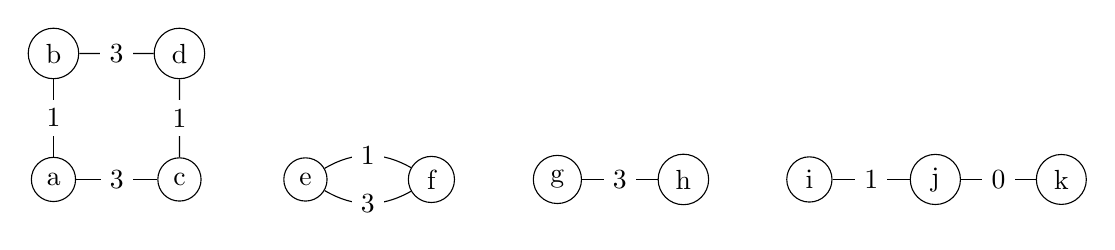
\begin{tikzpicture}[scale=.8]

        \begin{scope}[every node/.style={circle,draw}]
          \node (1)  at (0,2)  {b};
          \node (2)  at (0,0)  {a};
          \node (3)  at (2,2)  {d};
          \node (4)  at (2,0)  {c};
          \node (5)  at (4,0)  {e};
          \node (6)  at (6,0)  {f};
          \node (7)  at (14,0) {j};
          \node (8)  at (12,0) {i};
          \node (9)  at (8,0)  {g};
          \node (10) at (10,0) {h};
          \node (11) at (16,0) {k};
        \end{scope}

        \begin{scope}[every node/.style={fill=white}]

          \begin{scope}[every edge/.style={draw}]
            \path (7)  edge node {$0$} (11);
            \path (1)  edge node {$1$} (2);
            \path (3)  edge node {$1$} (4);
            \path (5)  edge[bend left=30] node {$1$} (6);
            \path (7)  edge node {$1$} (8);
            \path (1)  edge node {$3$} (3);
            \path (2)  edge node {$3$} (4);
            \path (5)  edge[bend right=30] node {$3$} (6);
            \path (9)  edge node {$3$} (10);
          \end{scope}
        \end{scope}

      \end{tikzpicture}
      \caption{}
    \end{center}
  \end{figure}

  \paragraph{}The other $\rho_0$ cannot connect different components by Propositions~\ref{chain-consecutive}, \ref{square-connection} and~\ref{adjacent-double}. Thus it must double an edge into a component.The component $\{i,j,k\}$ cannot be used because there is already a $\rho_0$ edge. If the edge is placed in the component $\{e,f\}$, then this component must be part of an alternating square by Proposition~\ref{continue-triple-edge}. The only available involution to make this alternating square is $\rho_2$. This new component then cannot be linked by $\rho_2$ edges\footnote{Graph}.

  \paragraph{}
  Thus the last $\rho_0$ edge must be used in the $\{a,b,c,d\}$ component.

  \begin{figure}[H]
    \begin{center}
      \begin{tikzpicture}[scale=.8]

        \begin{scope}[every node/.style={circle,draw}]
          \node (1)  at (0,2)  {};
          \node (2)  at (0,0)  {};
          \node (3)  at (2,2)  {};
          \node (4)  at (2,0)  {};
          \node (5)  at (4,0)  {};
          \node (6)  at (6,0)  {};
          \node (7)  at (14,0)  {};
          \node (8)  at (12,0)  {};
          \node (9)  at (8,0)  {};
          \node (10) at (10,0)  {};
          \node (11) at (16,0) {};
        \end{scope}

        \begin{scope}[every node/.style={fill=white}]

          \begin{scope}[every edge/.style={draw}]
            \path (1)  edge[bend left=30] node {$0$} (3);
            \path (7)  edge node {$0$} (11);
            \path (1)  edge node {$1$} (2);
            \path (3)  edge node {$1$} (4);
            \path (5)  edge[bend left=30] node {$1$} (6);
            \path (7)  edge node {$1$} (8);
            \path (1)  edge[bend right=30] node {$3$} (3);
            \path (2)  edge node {$3$} (4);
            \path (5)  edge[bend right=30] node {$3$} (6);
            \path (9)  edge node {$3$} (10);
          \end{scope}
        \end{scope}

      \end{tikzpicture}
      \caption{}
    \end{center}
  \end{figure}

  \paragraph{}
  There are only 4 $\rho_2$ edges to be placed. Three of them must link the components because there is only one "joker" edge remaining. There are multiple ways to link those components. As for the previous section, all the permutation representation graphs are displayed in Appendix~\ref{rank4-3-4transpositions}. We only consider one case but the reader can check that all the following statements can be applied to all other variants.

  \begin{figure}[H]
    \begin{center}
      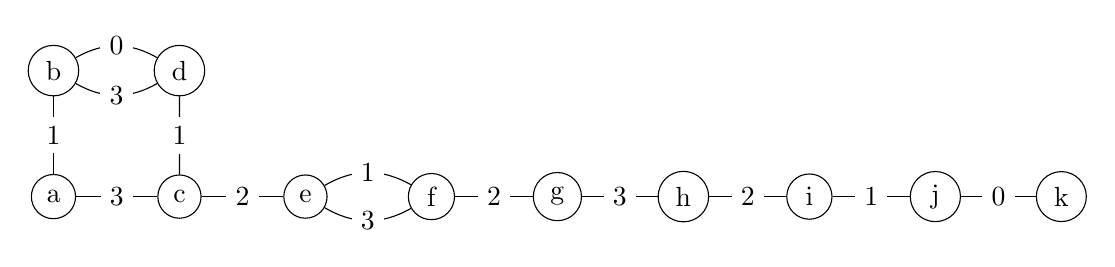
\begin{tikzpicture}[scale=.8]

        \begin{scope}[every node/.style={circle,draw}]
          \node (1)  at (0,2)  {b};
          \node (2)  at (0,0)  {a};
          \node (3)  at (2,2)  {d};
          \node (4)  at (2,0)  {c};
          \node (5)  at (4,0)  {e};
          \node (6)  at (6,0)  {f};
          \node (7)  at (14,0)  {j};
          \node (8)  at (12,0)  {i};
          \node (9)  at (8,0)  {g};
          \node (10) at (10,0)  {h};
          \node (11) at (16,0) {k};
        \end{scope}

        \begin{scope}[every node/.style={fill=white}]

          \begin{scope}[every edge/.style={draw}]
            \path (1)  edge[bend left=30] node {$0$} (3);
            \path (7)  edge node {$0$} (11);
            \path (1)  edge node {$1$} (2);
            \path (3)  edge node {$1$} (4);
            \path (5)  edge[bend left=30] node {$1$} (6);
            \path (7)  edge node {$1$} (8);
            \path (4)  edge node {$2$} (5);
            \path (6)  edge node {$2$} (9);
            \path (10) edge node {$2$} (8);
            \path (1)  edge[bend right=30] node {$3$} (3);
            \path (2)  edge node {$3$} (4);
            \path (5)  edge[bend right=30] node {$3$} (6);
            \path (9)  edge node {$3$} (10);
          \end{scope}
        \end{scope}

      \end{tikzpicture}
      \caption{}
    \end{center}
  \end{figure}

  \paragraph{}
  The last $\rho_2$ edge must double something. The only two possibilities are: triple the double edge $(b, d)$ or double the edge $(j,k)$.

  \paragraph{}
  If the edge $(j,k)$ is doubled, the graph is the following:

  \begin{figure}[H]
    \begin{center}
      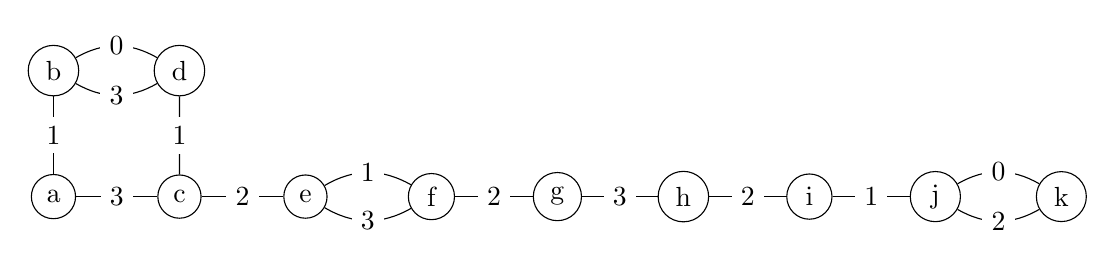
\begin{tikzpicture}[scale=.8]

        \begin{scope}[every node/.style={circle,draw}]
          \node (1)  at (0,2)  {b};
          \node (2)  at (0,0)  {a};
          \node (3)  at (2,2)  {d};
          \node (4)  at (2,0)  {c};
          \node (5)  at (4,0)  {e};
          \node (6)  at (6,0)  {f};
          \node (7)  at (14,0)  {j};
          \node (8)  at (12,0)  {i};
          \node (9)  at (8,0)  {g};
          \node (10) at (10,0)  {h};
          \node (11) at (16,0) {k};
        \end{scope}

        \begin{scope}[every node/.style={fill=white}]

          \begin{scope}[every edge/.style={draw}]
            \path (1)  edge[bend left=30] node {$0$} (3);
            \path (7)  edge[bend left=30] node {$0$} (11);
            \path (1)  edge node {$1$} (2);
            \path (3)  edge node {$1$} (4);
            \path (5)  edge[bend left=30] node {$1$} (6);
            \path (7)  edge node {$1$} (8);
            \path (4)  edge node {$2$} (5);
            \path (6)  edge node {$2$} (9);
            \path (10) edge node {$2$} (8);
            \path (7) edge[bend right=30] node {$2$} (11);
            \path (1)  edge[bend right=30] node {$3$} (3);
            \path (2)  edge node {$3$} (4);
            \path (5)  edge[bend right=30] node {$3$} (6);
            \path (9)  edge node {$3$} (10);
          \end{scope}
        \end{scope}

      \end{tikzpicture}
      \caption{}
    \end{center}
  \end{figure}

  \paragraph{}
  We prove now that, in this case, $\rho_0$ can be written as a product of the other generators. If the $\rho_1$ edges are removed the graph becomes this one (for every variant too):

  \begin{figure}[H]
    \begin{center}
      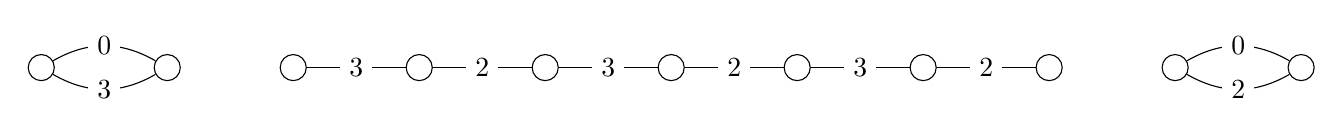
\begin{tikzpicture}[scale=.8]

        \begin{scope}[every node/.style={circle,draw}]
          \node (1)  at (-4,0)  {};
          \node (2)  at (-2,0)  {};
          \node (3)  at (14,0)  {};
          \node (4)  at (16,0) {};
          \node (5)  at (8,0)  {};
          \node (6)  at (10,0)  {};
          \node (7)  at (0,0)  {};
          \node (8)  at (2,0)  {};
          \node (9)  at (4,0)  {};
          \node (10) at (6,0)  {};
          \node (11) at (12,0)  {};
        \end{scope}

        \begin{scope}[every node/.style={fill=white}]

          \begin{scope}[every edge/.style={draw}]
            \path (1)  edge[bend left=30] node {$0$} (2);
            \path (3)  edge[bend left=30] node {$0$} (4);
            \path (3)  edge[bend right=30] node {$2$} (4);
            \path (5)  edge node {$2$} (10);
            \path (6)  edge node {$2$} (11);
            \path (8)  edge node {$2$} (9);
            \path (1)  edge[bend right=30] node {$3$} (2);
            \path (5)  edge node {$3$} (6);
            \path (7)  edge node {$3$} (8);
            \path (9)  edge node {$3$} (10);
          \end{scope}
        \end{scope}

      \end{tikzpicture}
      \caption{}
    \end{center}
  \end{figure}

  \paragraph{}
  It is clear here that $\rho_0 = (\rho_2 \rho_3)^7$. Thus the last $\rho_2$ edge must triple an existing double edge. Therefore the last $\rho_2$ edge must be $(b,d)$.

  \begin{figure}[H]
    \begin{center}
      \begin{tikzpicture}[scale=.8]

        \begin{scope}[every node/.style={circle,draw}]
          \node (1)  at (2,2)  {};
          \node (2)  at (0,2)  {};
          \node (3)  at (14,0)  {};
          \node (4)  at (16,0) {};
          \node (5)  at (8,0)  {};
          \node (6)  at (10,0)  {};
          \node (7)  at (0,0)  {};
          \node (8)  at (2,0)  {};
          \node (9)  at (4,0)  {};
          \node (10) at (6,0)  {};
          \node (11) at (12,0)  {};
        \end{scope}

        \begin{scope}[every node/.style={fill=white}]

          \begin{scope}[every edge/.style={draw}]
            \path (1)  edge[bend right=45] node {$0$} (2);
            \path (3)  edge node {$0$} (4);
            \path (1)  edge node {$1$} (8);
            \path (2)  edge node {$1$} (7);
            \path (3)  edge node {$1$} (11);
            \path (9)  edge[bend left=30] node {$1$} (10);
            \path (1)  edge node {$2$} (2);
            \path (5)  edge node {$2$} (10);
            \path (6)  edge node {$2$} (11);
            \path (8)  edge node {$2$} (9);
            \path (1)  edge[bend left=45] node {$3$} (2);
            \path (5)  edge node {$3$} (6);
            \path (7)  edge node {$3$} (8);
            \path (9)  edge[bend right=30] node {$3$} (10);
          \end{scope}
        \end{scope}

      \end{tikzpicture}
      \caption{}
    \end{center}
  \end{figure}

\end{proof}

\begin{theorem}
  \label{rank4-3-th2}
  None of the sggis represented by the graphs in Appendix~\ref{rank4-2-4transpositions} are C-groups representations.
\end{theorem}

\begin{proof}
  As for previous similar proof, only the summary is displayed and the details is left to the reader.

  \begin{table}[H]
    \centering
    \begin{tabular}{|c|c|c|c|c|c|c|}
      \hline
      Figure & $\Gamma_{S_1}$ & $\Gamma_{S_2}$ & $\Gamma_{S_1 \cap S_2}$ & $\#\Gamma_{S_1 \cap S_2}$ & $\Gamma_{S_1} \cap \Gamma_{S_2}$ & $\#(\Gamma_{S_1} \cap \Gamma_{S_2})$ \\ \hline

      \ref{r4-5-1} & $S_7 : D_8$ & $A_{10}$ & $D_{42}$ & 42 & $\ge S_5$ & $\ge 120$ \\ \hline
      \ref{r4-5-2} & $A_{10}$ & $A_{10}$ & $D_{18}$ & 18 & $\ge A_9$ & $\ge 181440$ \\ \hline
      \ref{r4-5-3} & $A_{10}$ & $A_{10}$ & $D_{18}$ & 18 & $\ge A_9$ & $\ge 181440$ \\ \hline
      \ref{r4-5-4} & $S_7 : D_8$ & $A_{10}$ & $D_{42}$ & 42 & $\ge A_6$ & $\ge 360$ \\ \hline
      \ref{r4-5-5} & $A_5 : S_6$ & $A_{10}$ & $D_{10}$ & 10 & $\ge A_6$ & $\ge 360$ \\ \hline
      \ref{r4-5-6} & $A_8 : S_3$ & $A_{10}$ & $D_{42}$ & 42 & $\ge A_7$ & $\ge 2520$ \\ \hline

    \end{tabular}
  \end{table}
\end{proof}
